% Teilauswertung 1

\section{Einfluss der Messmethode }
\label{sec:mess}

\subsection{Verlauf der Reflexions- und Transmissionsmessung}
\label{sub:verlauf}

Zuerst wird der Einfluss der Konzentrationsvariation auf die Reflexion und Transmission untersucht. 
Dabei wird der Verlauf beider Messungen graphisch dargestellt in Abb. \ref{fig:reflexionVerlauf} den der Reflexionsmessung und in Abb. \ref{fig:transmissionVerlauf} den der Transmissionsmessung. Um die verläufe graphisch darzustellen wurde aus allen 6 Messungen der gleiche Bereich ausgewählt und der Mittelwert über die Amplitude des Signals gebildet.
\begin{center}
	\captionsetup{type=figure}
	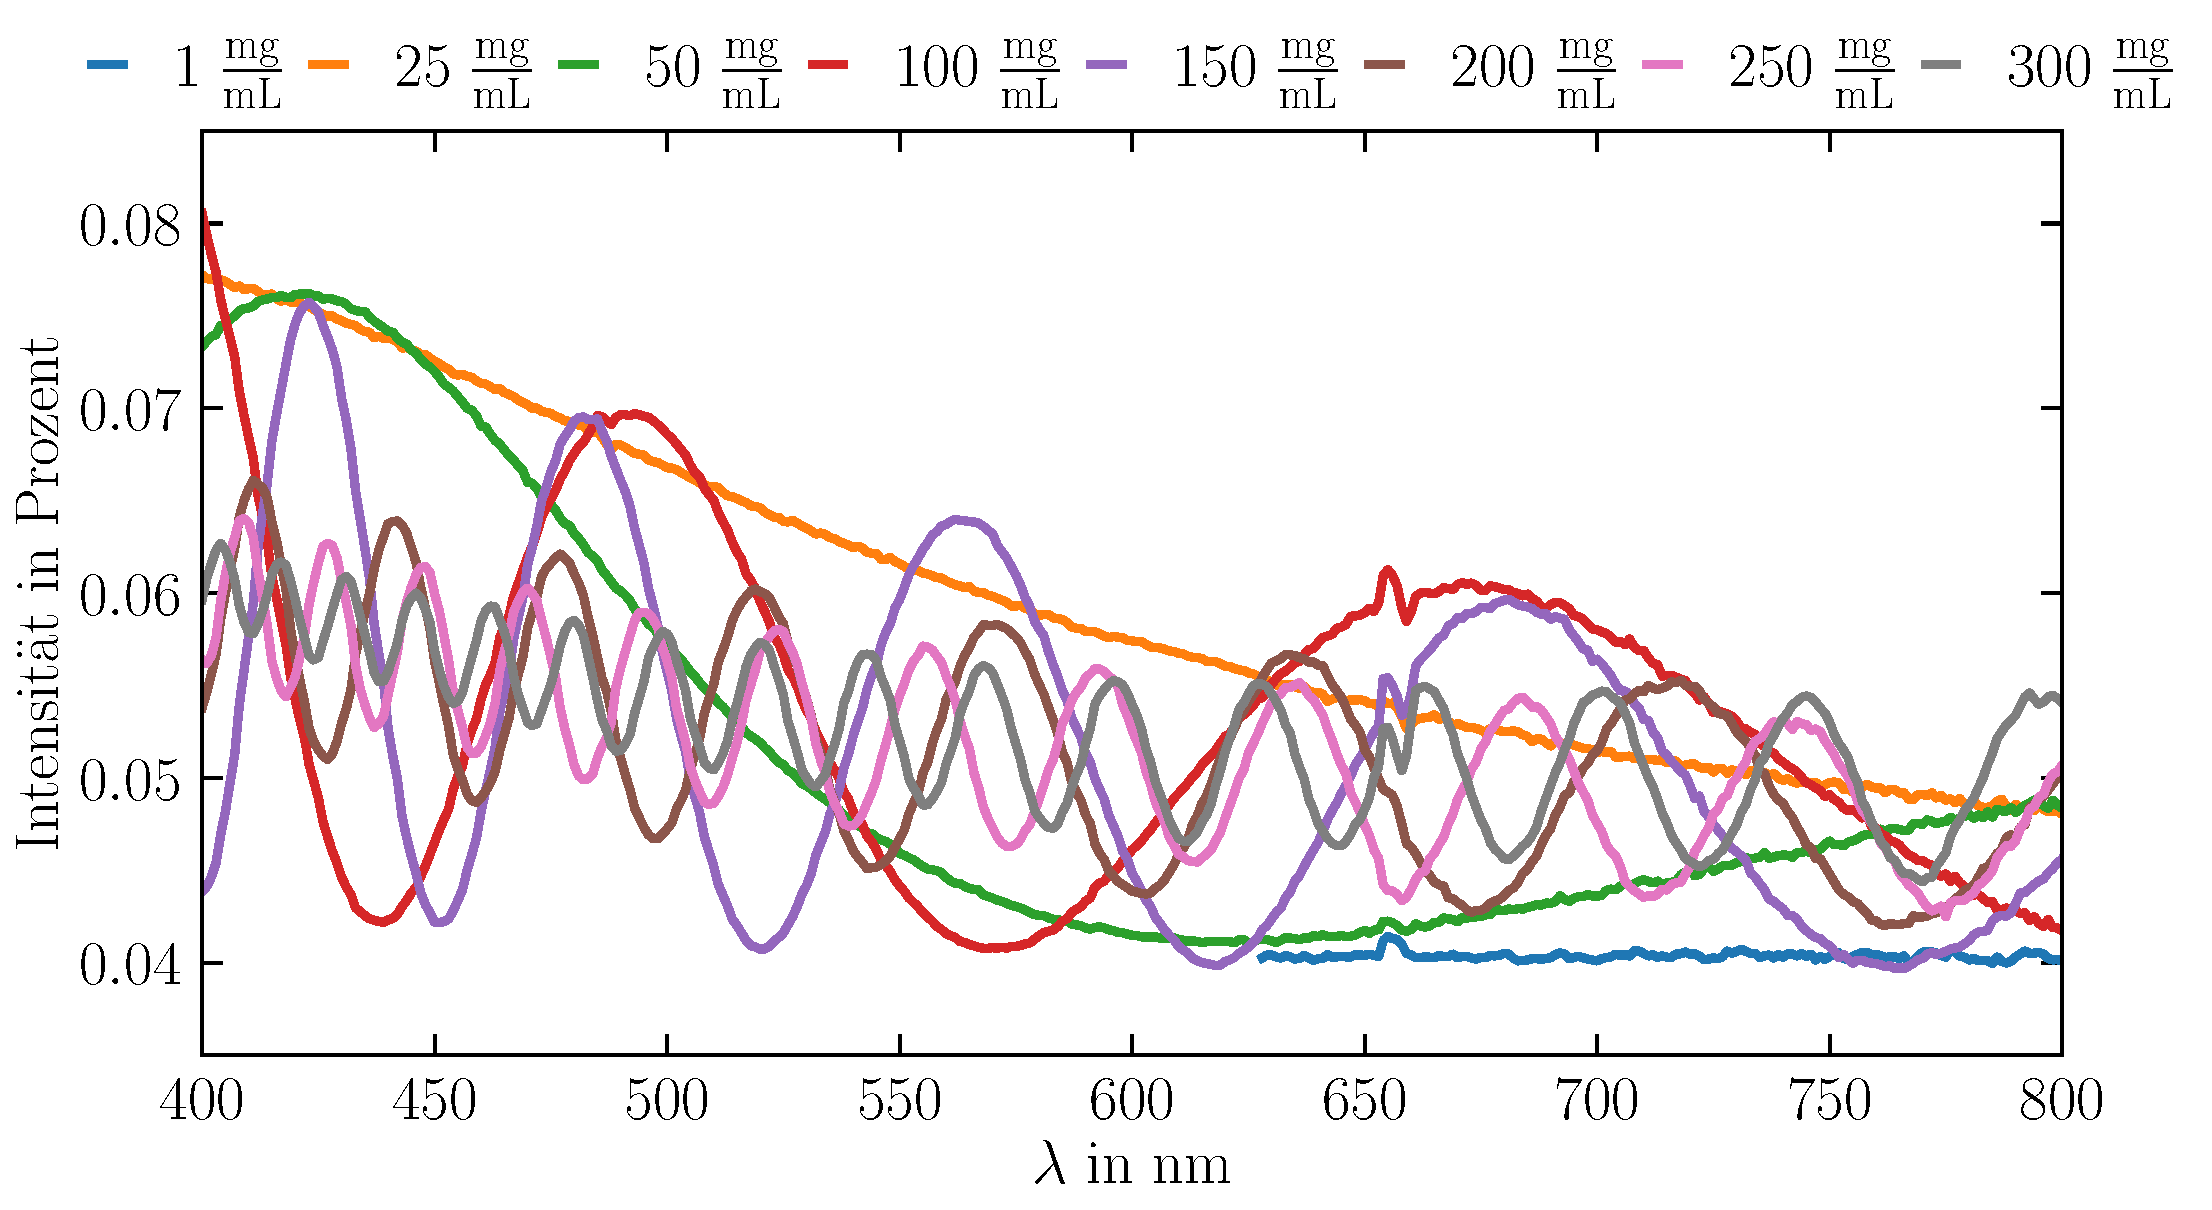
\includegraphics[width=\textwidth]{Auswertung/41/Reflexion.pdf}
	\captionof{figure}{Verlauf der Reflexionsmessung}
	\label{fig:reflexionVerlauf}
\end{center}
Mit Gleichung \ref{eq:wavelength} lässt sich schlussfolgern, dass die Schichtdicke mit zunehmender Konzentration zunimmt. Dies wird verdeutlicht, wenn man die Differenz zweier benachbarten Maximas im Spektrum. Dafür stellen wir Gleichung \ref{eq:wavelength} der reflektierten Welle (mit transmittierter Welle analog) für die Beugungsordnung $m$ um:
\begin{gather}
	\left(m_1 + \frac{1}{2}\right) - \left(m_2 + \frac{1}{2}\right) = 2nd \left(\frac{1}{\lambda_1} - \frac{1}{\lambda_2}\right)~.
\end{gather}
Da $m_1$ und $m_2$ benachbarte Maxima sind ergibt die Differenz einfach nur 1, zusammen mit dem Wellenlängenunterschied $\Delta \lambda = \lambda_2 - \lambda_1$ ergibt sich:
\begin{gather}
	\boxed{\frac{\lambda_1\lambda_2}{\Delta\lambda} = 2nd \Rightarrow d \xrightarrow{\Delta \lambda \rightarrow 0} \infty}~.
\end{gather} 
Dieser Zusammenhang zeigt, je kleiner der Wellenlängenunterschied $\Delta \lambda$ wird, desto größer ist die Schichtdicke $d$. Deswegen lässt sich aus Abb. \ref{fig:reflexionVerlauf} und Abb. \ref{fig:transmissionVerlauf} erkennen, dass mit zunehmender Konzentration die Schichtdicke $d$ zunimmt, da der Wellenlängenunterschied $\Delta \lambda$ kleiner wird.
\begin{center}
	\captionsetup{type=figure}
	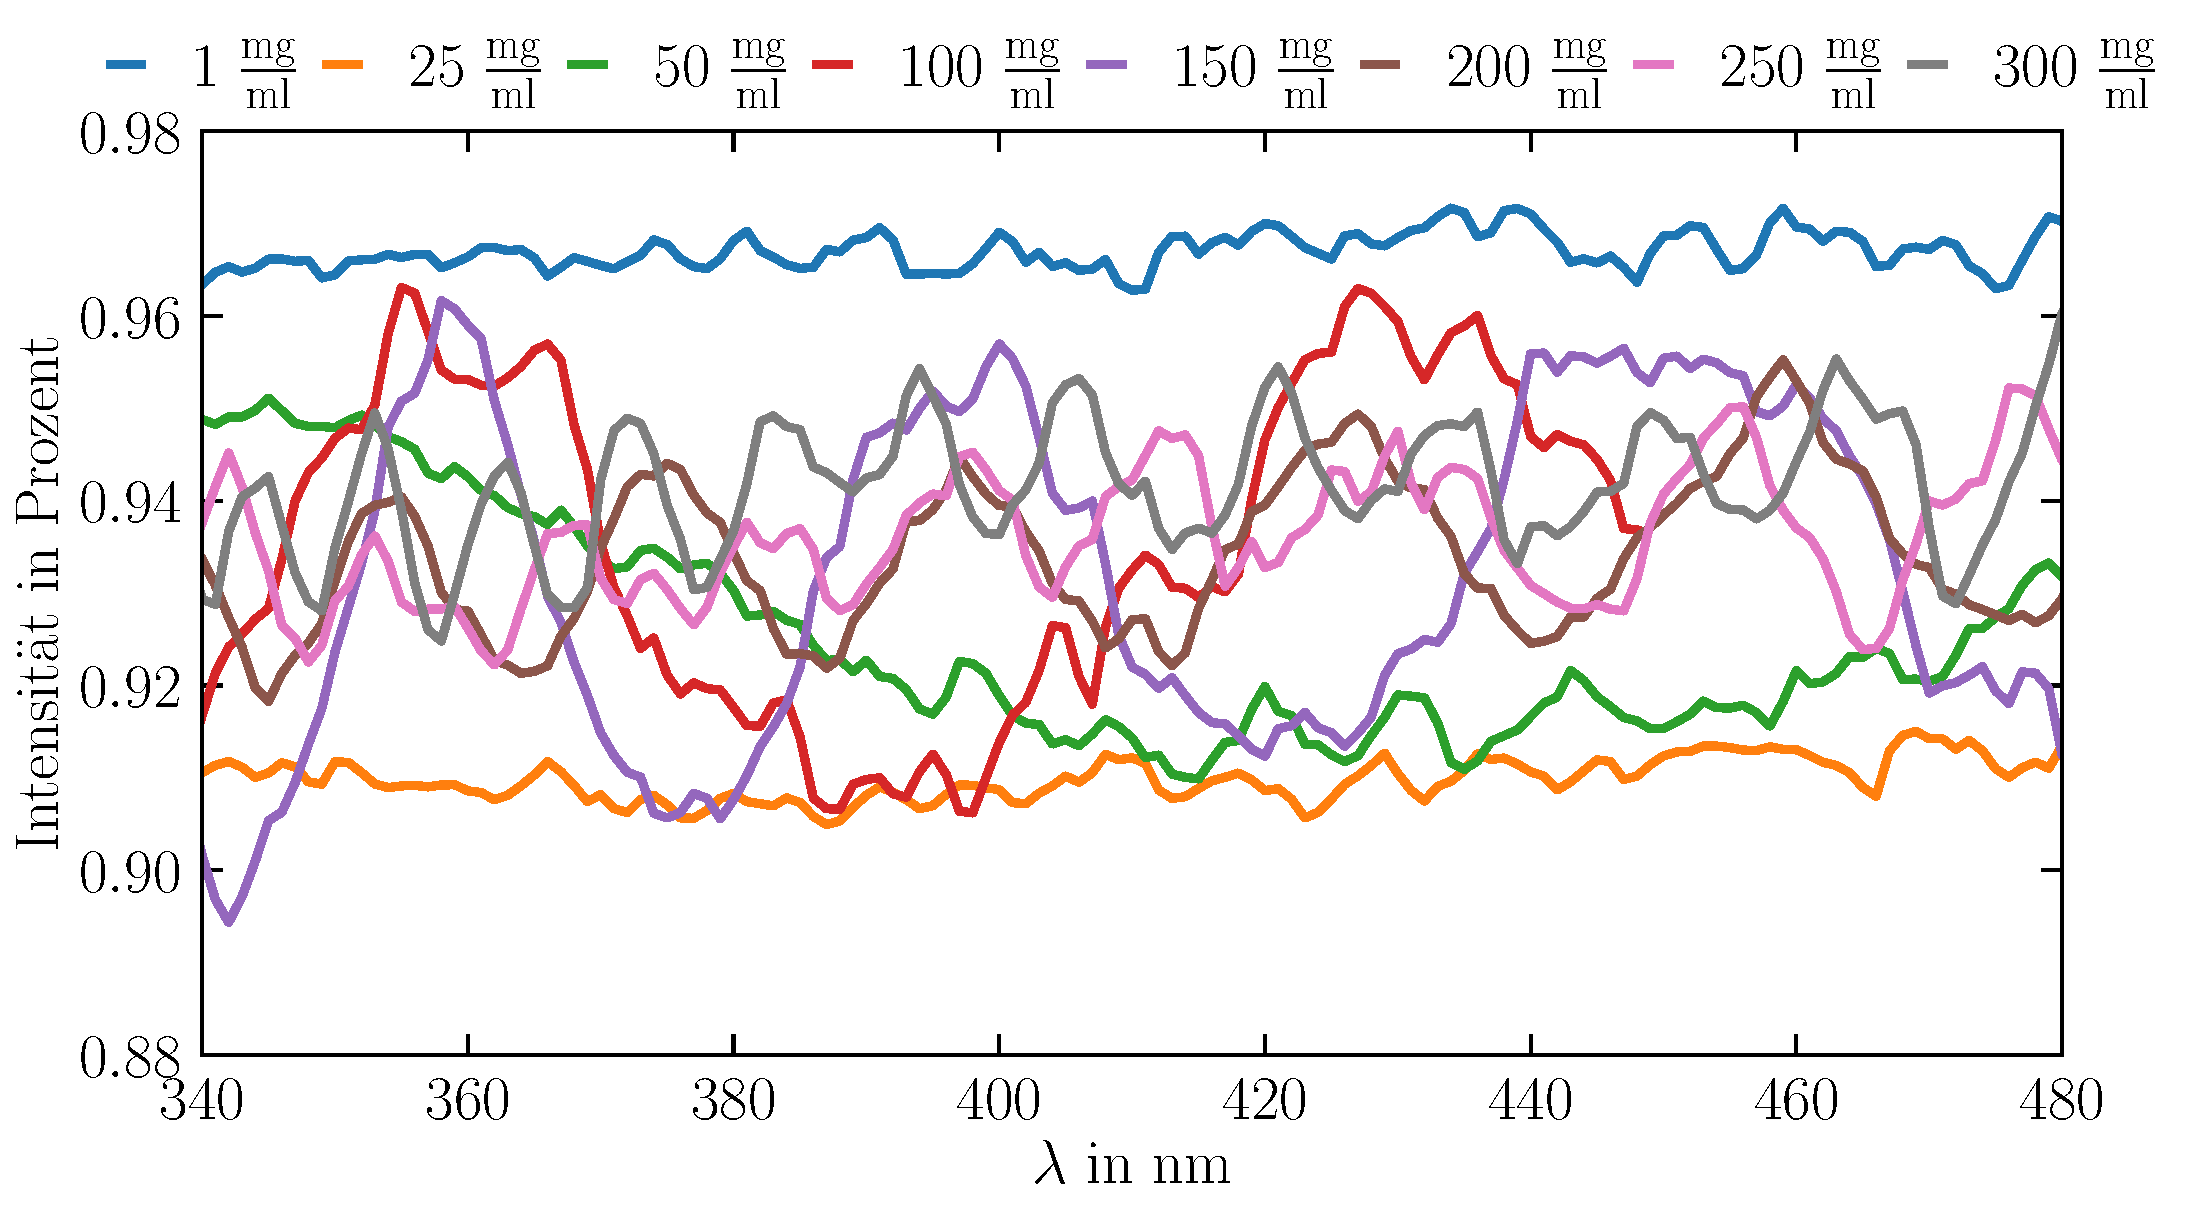
\includegraphics[width=\textwidth]{Auswertung/41/Transmission.pdf}
	\captionof{figure}{Verlauf der Transmissionsmessung}
	\label{fig:transmissionVerlauf}
\end{center}

\subsection{Hetrogenität $h$ der Probe}
\label{sub:fitguete}

Als nächstes betrachten wir die Heterogenität $h$ der Probe, um daraus die Homogenität dieser zu bestimmen. Dafür wir die Heterogenität $h$ mit folgender Formel berechnet:
\begin{gather}
	\boxed{h = \frac{\langle d \rangle}{std(d)}}~, 
\end{gather}
wobei $\langle d \rangle$ der Mittelwert und $std(d)$ die Standardabweichung der Schichtdicke $d$ für jede einzelne Probe ist. Als Werte für die Statistik werden die aufgenommenen Daten des NanoCalc Programms verwendet. Weiterhin wird auch die Fitgüte $\chi$ aus den Programm auch gemittelt ($\langle\chi\rangle)$. Die Ergebnisse werden in Tab. \ref{tab:homogen} dargestellt und wurden mit der \textit{mean()} und \textit{std()} Funktion des \textit{python}-Modules \textit{pandas} berechnet. 
\begin{center}
	\captionsetup{type=table}
	\begin{tabular}{c}	
		\begin{tabular}{r | r r r | r}
			$c$/\si{\milli\gram\per\milli\litre} & $\langle d \rangle$/\si{\nano\metre} & $std(d)$/\si{\nano\metre} & $h$ & $\langle \chi \rangle$ \\[0,1cm]
			\hline
			300 & 3656.3 & 33.1 & 110.5 & 0.016024 \\
			250 & 2708.4 & 33.1 &  81.8 & 0.016509 \\
			200 & 1702.4 & 20.0 &  85.1 & 0.011317 \\
			150 &  975.0 &  3.7 & 263.5 & 0.007943 \\
			100 &  539.2 &  3.6 & 149.8 & 0.007949 \\
			 50 &   60.6 &  1.0 &  60.6 & 0.005747 \\
			 25 &   60.6 &  1.0 &  60.6 & 0.005688 \\
		\end{tabular} \\[2cm]
		\begin{tabular}{r | r r r | r}
			$c$/\si{\milli\gram\per\milli\litre} & $\langle d \rangle$/\si{\nano\metre} & $std(d)$/\si{\nano\metre} & $h$ & $\langle \chi \rangle$ \\[0,1cm]
			\hline
			300 & 3756.9 & 23.2 & 161.9 & 0.101230 \\
			250 & 2835.6 & 37.5 &  75.6 & 0.093220 \\
			200 & 1833.5 & 24.3 &  75.5 & 0.101994 \\
			150 &  981.4 &  5.3 & 185.2 & 0.203744 \\
			100 &  564.1 & 41.1 &  13.7 & 0.299021 \\
			 50 &  200.1 &  7.3 &  27.4 & 0.214980 \\
			 25 &   64.1 &  1.5 &  42.7 & 0.435492 \\
		\end{tabular} \\
	\end{tabular}
	\captionof{table}{Werte für Homogenität bei Reflexion (oben) und Transmission (unten)}
	\label{tab:homogen}
\end{center}
In Tab. \ref{tab:homogen} lässt durch die Heterogenität $h$ sehen, dass die Probe selber nur wenig homogen verteilt ist. Dies bedeutet, dass sich einige dichtere Stellen von Material auf der Probe gebildet haben. Jedoch je höher die Konzentration war, desto homogener wurde der Dünnfilm auf der Probe. Anzumerken ist noch, dass die Hetrogenität $h$ der Transmission am aussagekräftigsten ist, da für das Messsignal das Licht der Halogen-Deuterium-Lampe durch die ganze Probe laufen muss. \bigskip

\subsection{Schichtdicke $d$ der Proben im Vergleich zur Fitgüte $\chi$}
\label{sub:fitguete}

Im nächsten Schritt wird der Mittelwert der Fitgüte $\langle \chi \rangle$ mit den Mittelwert und der Schichtdicke $\langle d \rangle$ und der Standardabweichung der Schichtdicke  $std(d)$ verglichen. In Abb. \ref{fig:fitgueteReflexion} und Abb. \ref{fig:fitueteTransmission} wird dieser Zusammenhang graphisch mit den Werten aus Tab. \ref{tab:homogen} dargestellt. Dabei lässt sich erkennen, dass bei der Reflexion die Verläufe linearer Proportionalität und bei der Transmission indirekter Proportionalität sind. Ein Fit mit der \textit{curve\_fit()} Funktion aus dem \textit{python}-Modules \textit{scipy.optimize} ergibt dann folgende Werte in Tab. \ref{tab:fitgueteFit}
\begin{center}
	\captionsetup{type=table}
	\begin{tabular}{l | c c | c c}
		  & \multicolumn{2}{c |}{Reflexion} &\multicolumn{2}{c}{Tranmission} \\
		  & $\langle \chi \rangle = a\,\langle d \rangle  + b$ & $\langle \chi \rangle = a\,std(d)  + b$ & $\langle \chi \rangle = a/\langle d \rangle^2 + b$ & $\langle \chi \rangle = a/std(d)^2 + b$\\
		  \hline
		  $a$/\si{\per\nano\metre} & 0.000003 & 0.000304 &  1.34 &  0.77 \\
		  $b$                      & 0.005714 & 0.006008 & -0.39 & -0.36 \\
	\end{tabular}
	\captionof{table}{Ermittelte Fitparameter für Reflexion- und Transmissionsmessung}
	\label{tab:fitgueteFit}
\end{center}
Es zeigt sich, dass die Fitgüte $\chi$ je nach Art der Messung verschieden skaliert abhängig von der Konzentration auf der Probe und damit der Schichtdicke $d$. \\
Dabei weißen Reflexion und Transmission gegenläufige Ergebnisse auf, dass sich sich in den Verläufen in Abb. \ref{fig:fitgueteReflexion} und Abb. \ref{fig:fitueteTransmission} erkennen lässt. Für die Reflexion ist hierbei die Fitgüte $\chi$ maximal, wenn die Schichtdicke $d$ groß ist, während für die Transmission die Fitgüte $\chi$ minimal ist für große Schichtdicken $d$. 
\begin{center}
	\captionsetup{type=figure}
	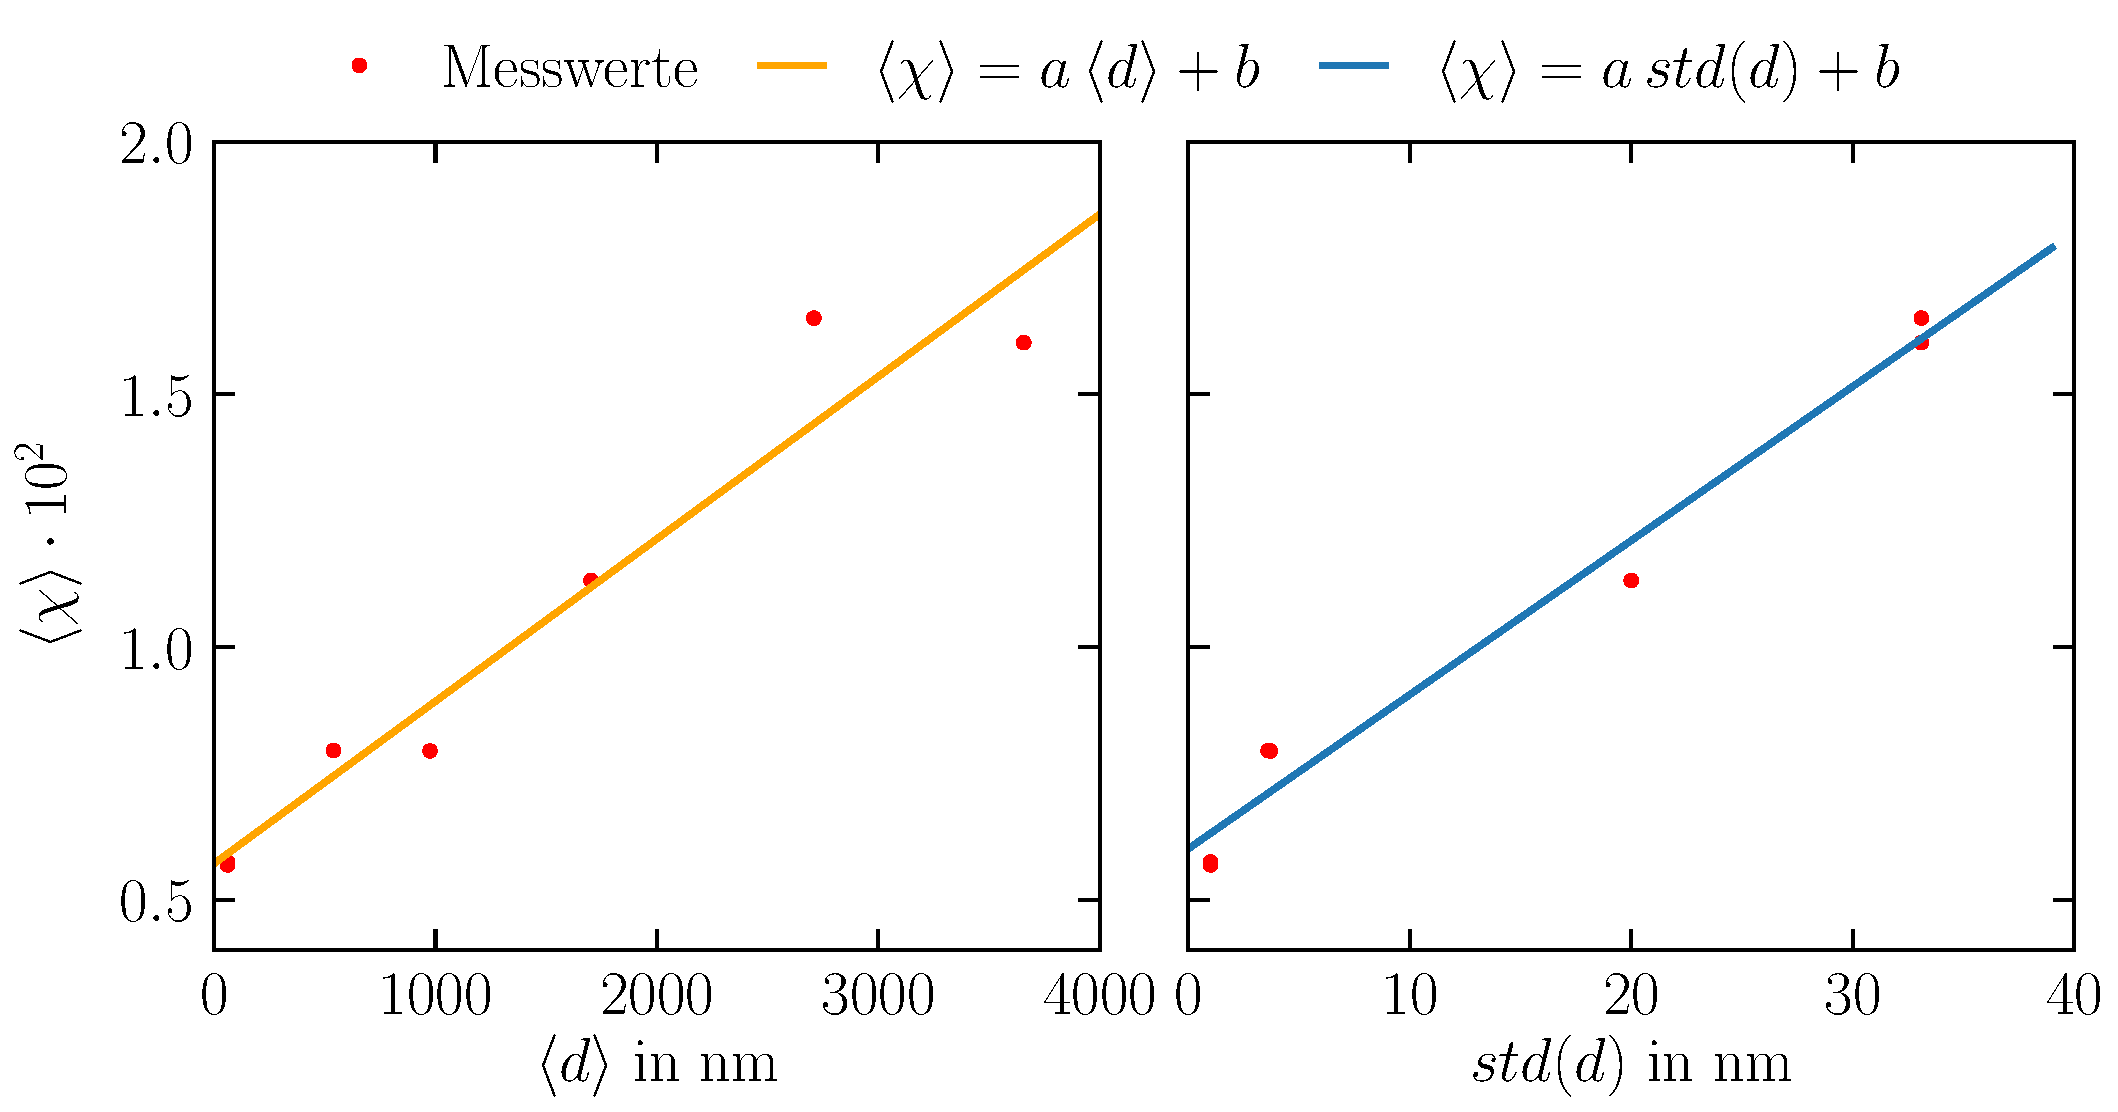
\includegraphics[width=0.92\textwidth]{Auswertung/41/Reflexion-Fitguete.pdf}
	\captionof{figure}{Mittelwert und Standardabweichung der Schichtdicke $d$ aufgetragen gegen den Mittelwert der Fitgüte $\langle \chi \rangle$ bei Reflexion}
	\label{fig:fitgueteReflexion}
\end{center}
\begin{center}
	\captionsetup{type=figure}
	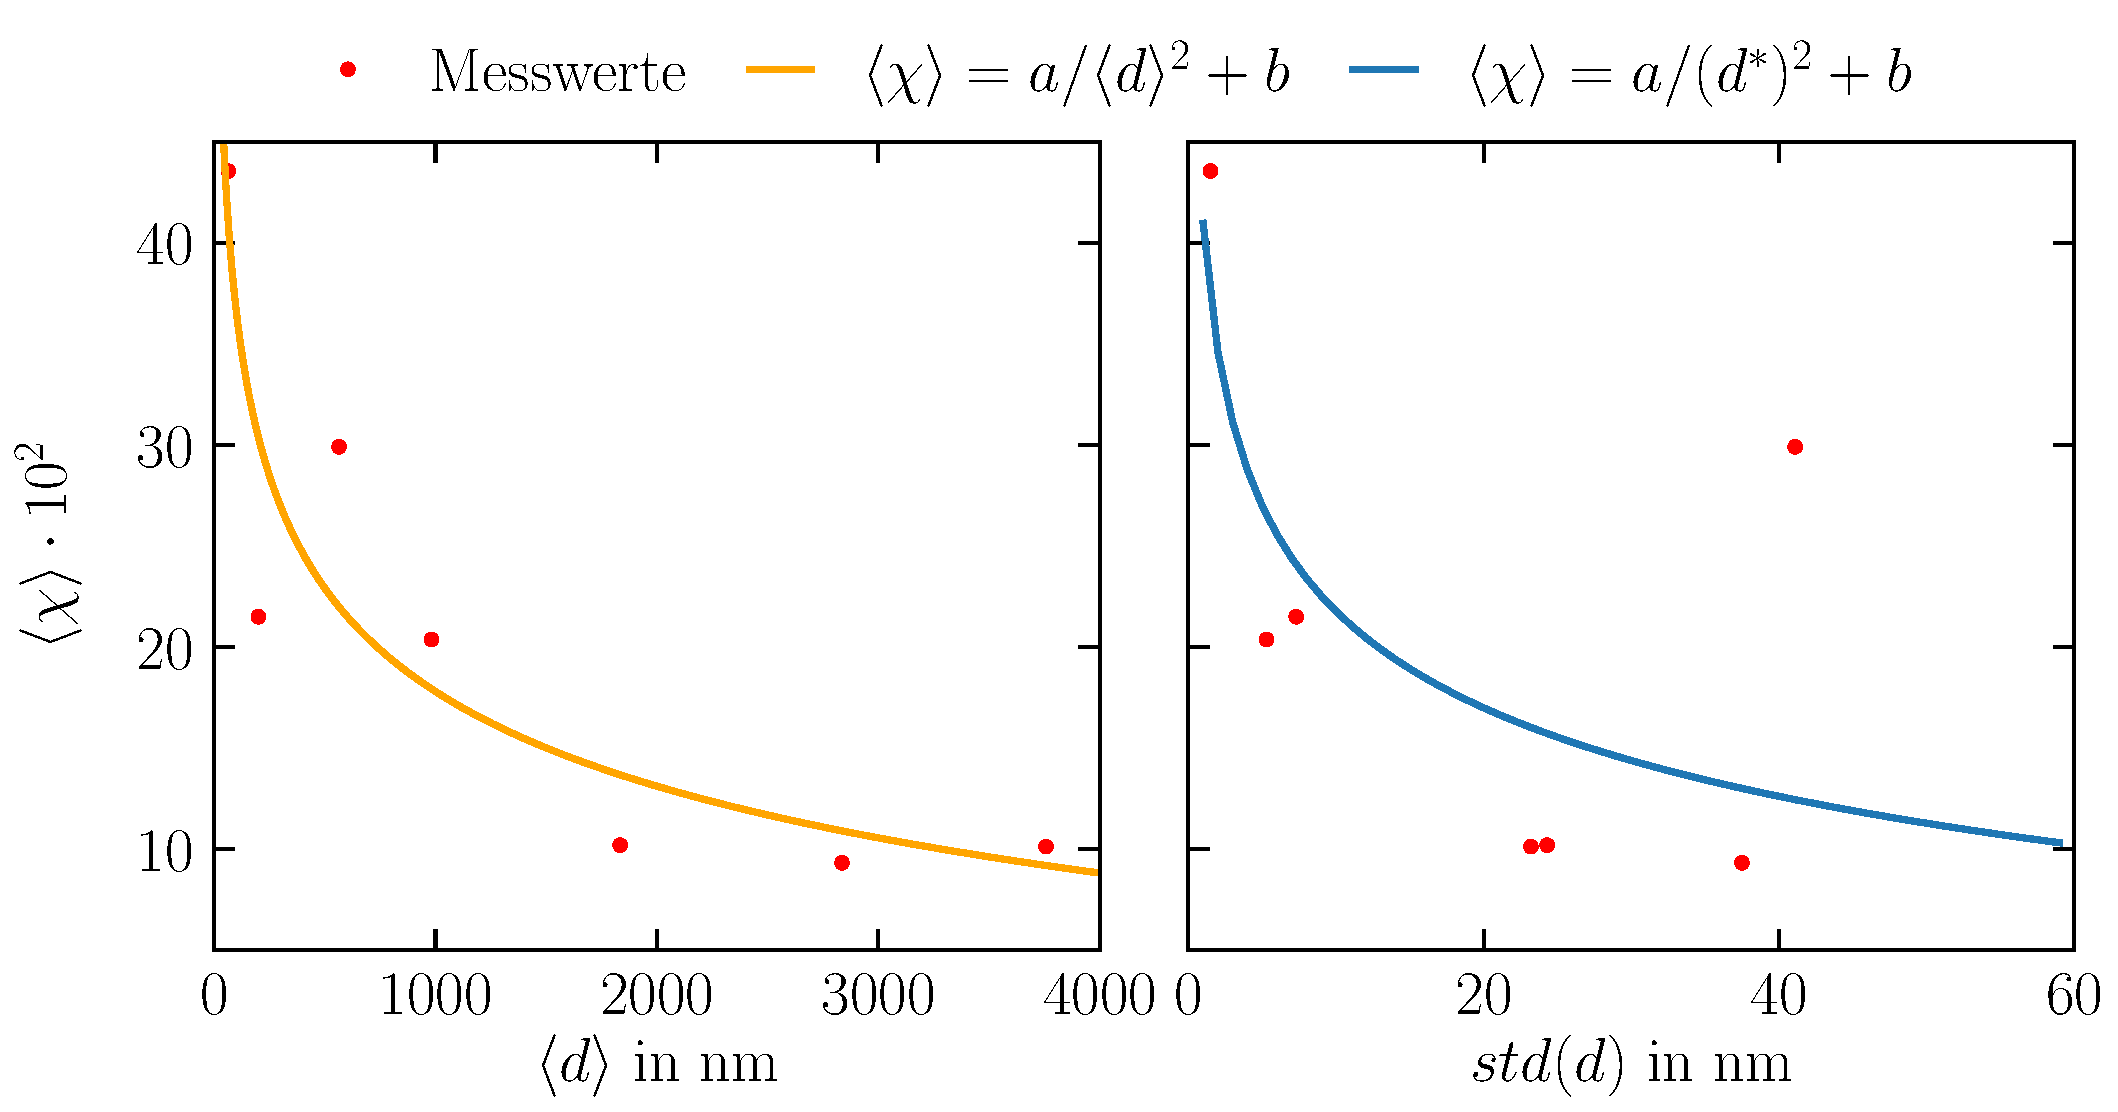
\includegraphics[width=0.92\textwidth]{Auswertung/41/Transmission-Fitguete.pdf}
	\captionof{figure}{Mittelwert und Standardabweichung der Schichtdicke $d$ aufgetragen gegen den Mittelwert der Fitgüte $\langle \chi \rangle$ bei Transmission}
	\label{fig:fitueteTransmission}
\end{center}


\subsection{Vergleich der Messmethoden}
\label{sub:vergleich}

Tab. \ref{tab:homogen} zeigt, dass bei Reflexion und Transmission ähnliche Werte für die Schichtdicke $d$ gemessen werden. Jedoch ist die Messung der Reflexion mit einem besseren Signal möglich als bei der Transmission [Fig. \ref{fig:reflexionVerlauf}, \ref{fig:transmissionVerlauf}]. Auch liefert die Reflexionsmessung einen linearen Zusammenhang [Fig. \ref{fig:fitgueteReflexion}] zwischen Fitgüte $\chi$ und der Schichtdicke $d$, was eine klare Prognose für die Fits der NanoCalc Software verspricht. Dennoch kann die Transmissionsmessung, dafür genutzt werden die Hetreogenität und damit die Homogenität der Probe zu bestimmen und ist der der Messung mit Reflexion vorzuziehen.